\chapter{Principali punti di estensione}

Il prodotto \textit{Login-warrior} realizzato dal gruppo è pensato in modo da poter attuare estesioni e manutenzioni in futuro. La manutenzione del codice è favorita dall'utilizzo di software di analisi statica, come ESLint, che permettono di mantenere il codice privo di errori e uno stile di codifica coerente tra i vari file.

\section{Aggiunta di un nuovo grafico}
Il prodotto permette di visualizzare diverse tipologie di grafici generati dai dati caricati, ed è possibile aggiungerne di nuove:
\begin{enumerate}
    \item Dalla directory principale spostarsi nella cartella in cui ci sono le varie pagine dei grafici seguendo il perorso \texttt{src\textbackslash login\_warrior\textbackslash src\textbackslash pages}. In questa posizione creare e spostarsi all'interno di una nuova cartella (e.g. "ScatterPlot3"), creare un file \textit{index.html} uguale a quello delle altre pagine a cui però si deve cambiare il titolo. Questa operazione serve per creare la struttura base per la visualizzazione del nuovo grafico;
    \begin{figure}[H]
        \centering
        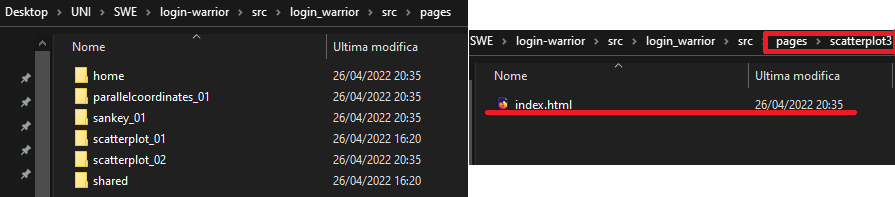
\includegraphics[width=\textwidth]{Passo1.png}
      \end{figure}

    \item Modificare il file \textit{index.html} presente nella cartella "home", raggiungibile seguendo il percorso \texttt{src\textbackslash login\_warrior\textbackslash src\textbackslash pages} dalla directory principale del progetto, aggiungendo un elemento "\#plot-entry" alla lista "\#plot-list", controllando di indicare il percorso corretto al nuovo grafico in ".plot-link". Questo passo permette di vedere la scelta del nuovo grafico inserito all'interno della lista di grafici disponibili nella homepage;
    \begin{figure}[H]
        \centering
        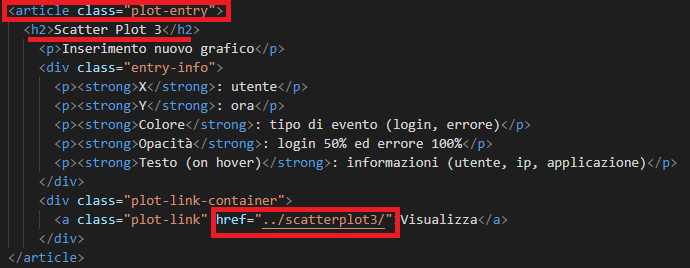
\includegraphics[width=\textwidth]{Passo2.png}
      \end{figure}

    \item Spostarsi nella cartella "drawers" seguendo il percorso \texttt{src\textbackslash login\_warrior\textbackslash src \textbackslash view\textbackslash drawers} dalla directory principale, creare una nuova classe che implementa l'interfaccia Drawer (e.g. ScatterPlot3). Questo passo permette di inserire i metodi necessari alla conversione del dataset in grafico;
    \begin{figure}[H]
        \centering
        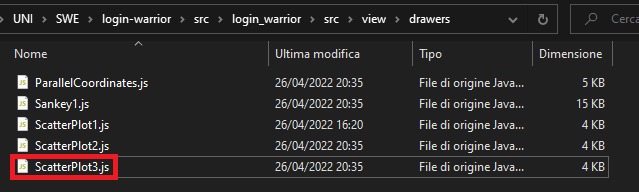
\includegraphics[width=\textwidth]{Passo3.png}
      \end{figure}

    \item Modificare il file "VisualizationView.js" seguendo il percorso \texttt{src\textbackslash login\_warrior \textbackslash src\textbackslash view} dalla cartella principale, nello specifico modificare lo switch del costruttore, aggiungendo un nuovo caso visualizationIndex (e.g. 5) e inizializzando la visualizzazione con il nuovo "Drawer"(e.g. ScatterPlot3). In questa fase è di fondamentale importanza importare il file presente nella cartella "drawers" creato nel punto precedente (e.g. \texttt{import ScatterPlot3 from ".\textbackslash drawers\textbackslash ScatterPlot3.js"}). Con questo passo si permette la visualizzazione del nuovo grafico nella lista dei grafici disponibili;
    \begin{figure}[H]
        \centering
        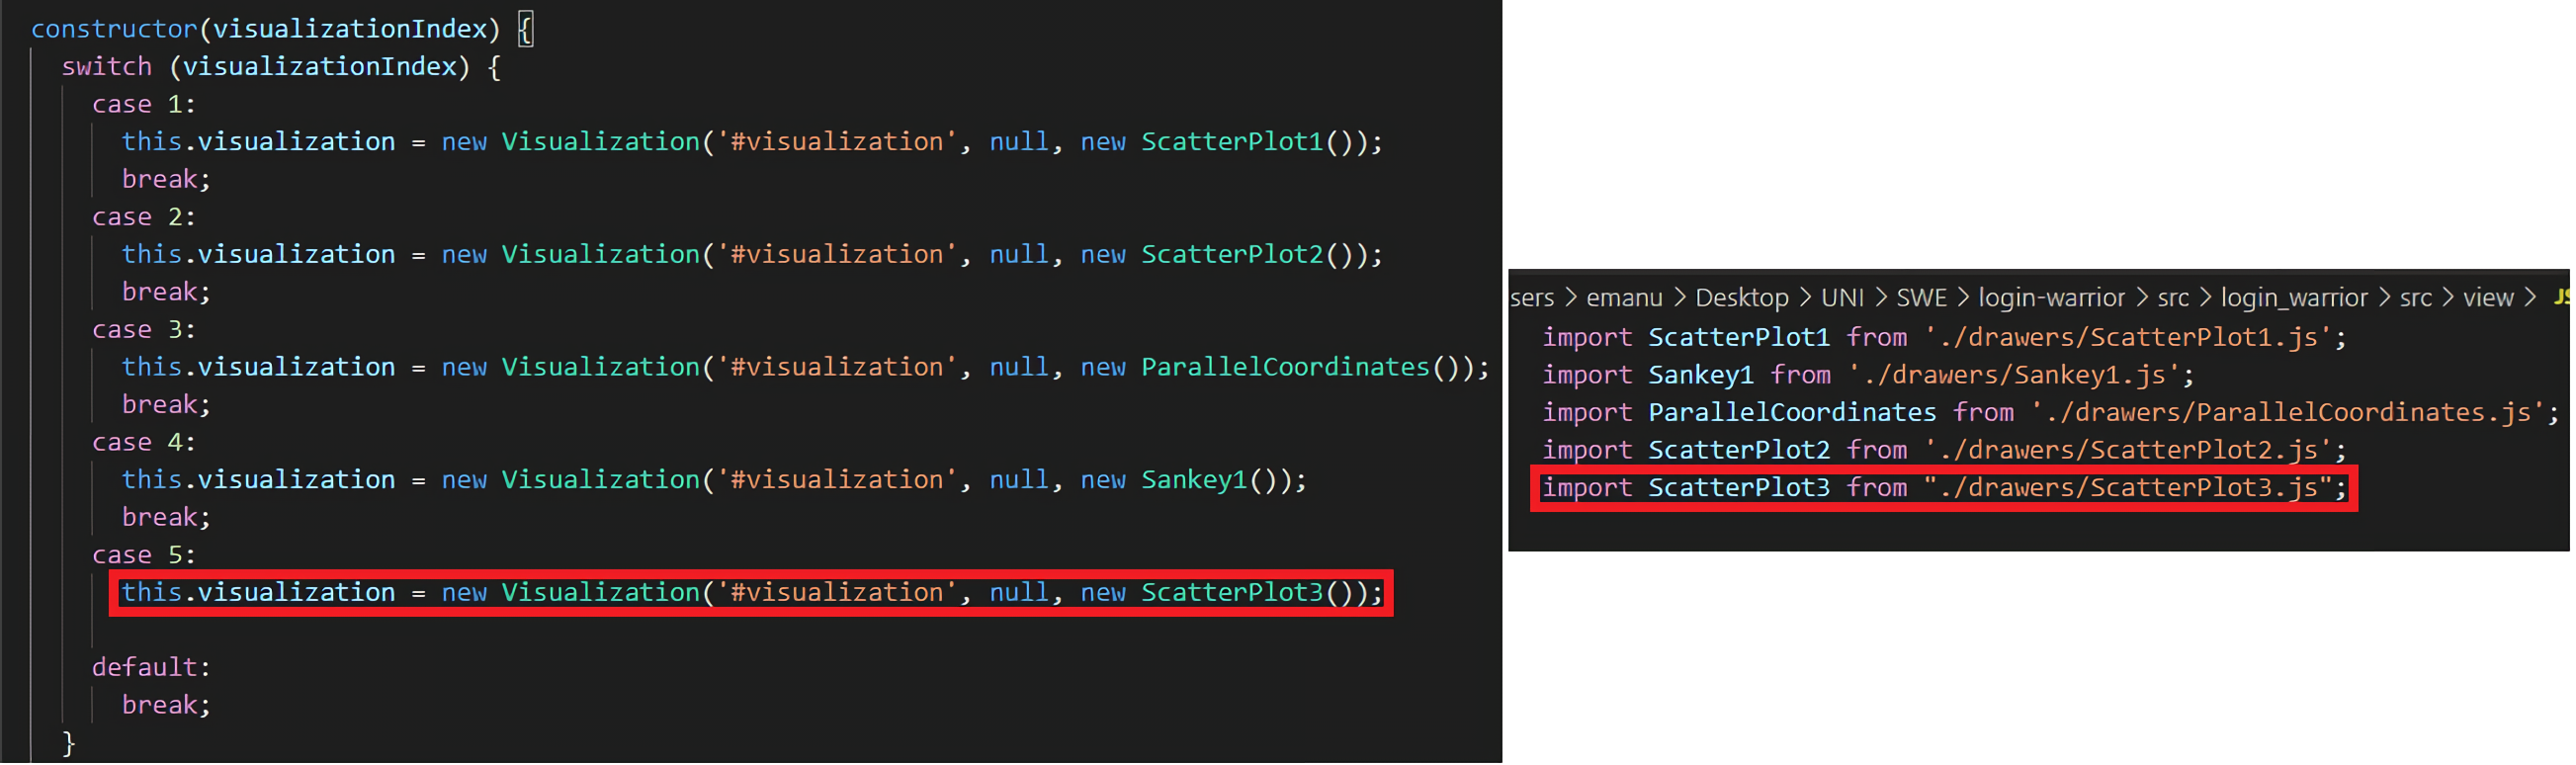
\includegraphics[width=\textwidth]{Passo4.png}
      \end{figure}

    \item Modificare il file "VisualizationsController.js" presente in \texttt{ src\textbackslash login\_warrior \textbackslash src\textbackslash controller} aggiornando il metodo "viewsInfo()" aggiungendo un caso allo switch con il nome della pagina della nuova visualizzazione (e.g. scatterplot3) e il rispettivo visualizationIndex specificato nel punto precedente (e.g. 5, che è stato definito in \texttt{src\textbackslash login\_warrior\textbackslash src\textbackslash view \textbackslash VisualizationView.js}). Come ultimo passo è necessario scegliere un numero massimo di punti per il campionamento andando a definire la variabile "samplesLimit". Con questo passo si va ad aggiornare il controller delle pagine che visualizzano i grafici, definendo le caratteristiche della nuova visualizzazione.
    \begin{figure}[H]
        \centering
        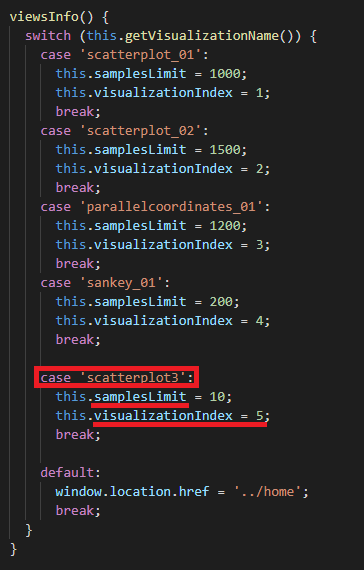
\includegraphics[scale=0.6]{Passo5.png}
      \end{figure}

    \item Come punto finale, se l'applicazione è stata utilizzata almeno una volta prima delle modifiche sopra riportate, pulire la cache del Browser utilizzato.
\end{enumerate}

\begin{figure}[H]
    \centering
    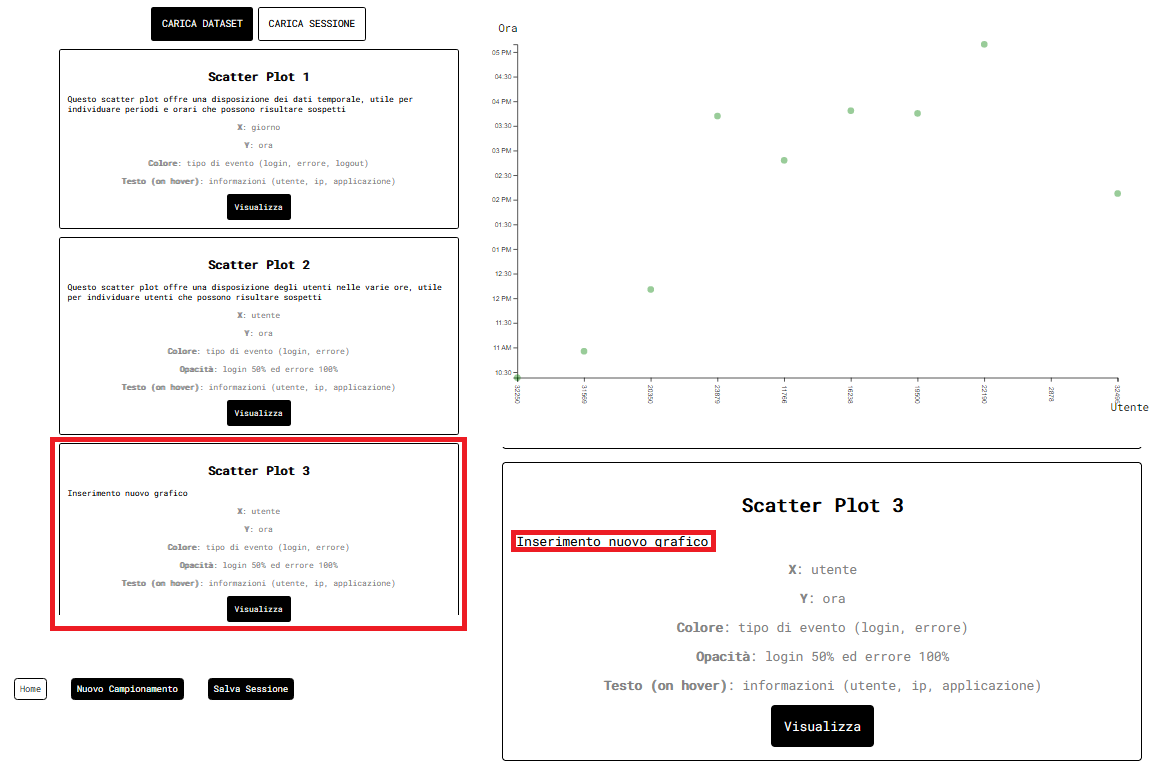
\includegraphics[width=\textwidth]{Passo6.png}
    \caption{Risultato dell'aggiunta del grafico}
  \end{figure}
